\documentclass[a4paper,twoside,10pt]{article}
\usepackage{a4wide,graphicx,fancyhdr,amsmath,amssymb}
\usepackage{algorithm}
\usepackage{algorithmic}
\usepackage{hyperref}
\usepackage{ragged2e}

%----------------------- Macros and Definitions --------------------------

\setlength\headheight{20pt}
\addtolength\topmargin{-10pt}
\addtolength\footskip{20pt}

\newcommand{\N}{\mathbb{N}}
\newcommand{\ch}{\mathcal{CH}}

\newcommand{\exercise}[2]{\noindent{\bf Question #1 (#2pt):} \\\\ }

\fancypagestyle{plain}{%
\fancyhf{}
\fancyhead[LO,RE]{\sffamily\bfseries\large Eindhoven University of Technology}
\fancyhead[RO,LE]{\sffamily\bfseries\large 2IMM10 Recommender Systems}
\fancyfoot[LO,RE]{\sffamily\bfseries\large Department of Mathematics and Computer Science}
\fancyfoot[RO,LE]{\sffamily\bfseries\thepage}
\renewcommand{\headrulewidth}{0pt}
\renewcommand{\footrulewidth}{0pt}
}

\pagestyle{fancy}
\fancyhf{}
\fancyhead[RO,LE]{\sffamily\bfseries\large Eindhoven University of Technology}
\fancyhead[LO,RE]{\sffamily\bfseries\large 2IMM10 Recommender Systems}
\fancyfoot[LO,RE]{\sffamily\bfseries\large Department of Mathematics and Computer Science}
\fancyfoot[RO,LE]{\sffamily\bfseries\thepage}
\renewcommand{\headrulewidth}{1pt}
\renewcommand{\footrulewidth}{0pt}

%-------------------------------- Title ----------------------------------

\title{\vspace{-\baselineskip}\sffamily\bfseries Assignment 3 \\
\large Deadline: Tuesday, April 13th (23.59)}
%\author{Puck Mulders \qquad Student number: 0737709 \\{\tt p.j.a.m.mulders@student.tue.nl}}

\date{\today}

%--------------------------------- Text ----------------------------------

\begin{document}
\maketitle

\section*{Question 1: Siamese networks (8pt)}
The Cifar-100 dataset is similar to the Cifar-10 dataset. It also consists of 60,000 32x32 RGB images, but they are distributed over 100 classes instead of 10. Thus, each class has much less examples, only 500 training images and 100 testing images per class. For more info about the dataset, see \url{https://www.cs.toronto.edu/~kriz/cifar.html}.

\emph{HINT: Import the Cifar-100 dataset directly from Keras, no need to download it from the website. Use} \texttt{label\_mode="fine"}

\subsection*{Task 1.1: Siamese network}
\begin{itemize}
	\item[a)] \begin{itemize}
		\item Train a Siamese Network on the first 80 classes of (the training set of) Cifar-100, i.e. let the network predict the probability that two input images are from the same class. Use 1 as a target for pairs of images from the same class (positive pairs), and 0 for pairs of images from different classes (negative pairs). Randomly select image pairs from Cifar-100, but make sure you train on as many positive pairs as negative pairs.
		\item Evaluate the performance of the network on 20-way one-shot learning tasks. Do this by generating 250 random tasks and obtain the average accuracy for each evaluation round. Use the remaining 20 classes that were not used for training. The model should perform better than random guessing.
		\end{itemize}
	For this question you may ignore the test set of Cifar-100; it suffices to use only the training set and split this, using the first 80 classes for training and the remaining 20 classes for one-shot testing.

	\emph{NOTE: do not expect the one-shot accuracy for Cifar-100 to be similar to that accuracy for Omniglot; a lower accuracy can be expected. However, accuracy higher than random guess is certainly achievable.}
	\item[b)] Briefly motivate your model's architecture, as well as its performance. What accuracy would random guessing achieve (on average)?
	\item[c)] Compare the performance of your Siamese network for Cifar-100 to the Siamese network from Practical 4 for Omniglot. Name three fundamental differences between the Cifar-100 and Omniglot datasets. How do these differences influence the difference in one-shot accuracy?
\end{itemize}

\subsection*{Task 1.2: One-shot learning with neural codes}
\begin{itemize}
	\item[a)] \begin{itemize}
		\item Train a CNN classifier on the first 80 classes of Cifar-100. Make sure it achieves at least 40\% classification accuracy on those 80 classes (use the test set to validate this accuracy).
		\item Then use neural codes from one of the later hidden layers of the CNN with L2-distance to evaluate one-shot learning accuracy for the remaining 20 classes of Cifar-100. I.e. for a given one-shot task, obtain neural codes for the test image as well as the support set. Then pick the image from the support set that is closest (in L2-distance) to the test image as your one-shot prediction.
	\end{itemize}
	\item[b)] Briefly motivate your CNN architecture, and discuss the difference in one-shot accuracy between the Siamese network approach and the CNN neural codes approach.
\end{itemize}


\section*{Question 2: Sequence classification model (8pt)}

Create a Recurrent Neural Networks (RNN) model by using words as input sequence. You need to complete three (3) main tasks as follows:

\begin{itemize}
    \item[-] Train and evaluate model on a binary classification task
    \item[-] Retrieve text features (document embedding) from recurrent layer of the model
    \item[-] Use the trained model to produce labels on unseen data set (one shot learning) 
\end{itemize}

\subsection*{Data description}

Raw text of IMDB review data set can be downloaded \href{https://storage.googleapis.com/trl_data/imdb_dataset.zip}{$[[$here$]]$}. You only need to use training and validation set to train and evaluate model. You can use the code from practical 5 to preprocess data.

\justify
For one shot learning task, two (2) data sets are used \href{https://storage.googleapis.com/trl_data/example1_labelled.tsv}{$[[$example1\_labelled$]]$}and \href{https://storage.googleapis.com/trl_data/example2_unlabelled.tsv}{$[[$example2\_unlabelled$]]$}. Both data sets are sampled from Amazon reviews of three (3) products: camera, laptop, mobile phone. The first data set contains three (3) instances (text reviews), i.e. one example per product category. The second data set is provided without labels. You can use the same preprocessing code that is used for IMDB data set.


\subsection*{Task 2.1: RNN model for text classification}

\begin{itemize}
  \item[a)] Train a model with RNN layer to classify sequence of words on a binary classification task (use Keras Functional API).

\justify  
For recurrent layer, compare four (4) different gate memory units:
    \begin{itemize}
       \item Long Short Term Memory (LSTM)
       \item Gated Recurrent Unit (GRU)
       \item Bidirectional LSTM 
       \item Bidirectional GRU
   \end{itemize}


\justify
\textbf{\textit{Note:}}   

\justify
Data set originally consists of $25.000$ training set and $25.000$ validation set. To improve training speed, you may consider to use smaller training and validation set. Be aware that the accuracy between $85$\%-$95$\% is plausible.
   
  \item[b)] Compare the model performance (loss, accuracy) of these 4 models (4 different gate units). 
  
  \begin{itemize}
      \item[-] Plot the model performance during training and validation stage. You shall have two (2) plots explaining the loss (training error vs. validation error) and accuracy (training accuracy vs. validation accuracy) for each model. Discuss the resulting plots.
      \item[-] Present the results, i.e. loss and accuracy on unseen validation set, in a comparison table.
  \end{itemize}
  
 
\end{itemize}

\subsection*{Task 2.2: Feature extraction}

\begin{itemize}
  \item[a)] Choose one model with the best performance from Task 2.1 and use that model to produce "Neural codes" (document embedding) of raw text (5000 instances of unseen validation set) from RNN layer.
  
  \item[b)] Use tSNE to reduce the dimension of extracted text features (encoded version of 5000 documents) into two (2) dimensions and visualize it towards their sentiment labels
  
\end{itemize}


\subsection*{Task 2.3: One shot learning on multi-class classification}

Consider the model you have trained on binary classification task (i.e. sentiment polarity of IMDB data set) as feature extractor. Define and implement an approach to assign labels on unlabelled set of reviews, by using the concept of "one shot learning". 

\begin{itemize}
    \item Discuss the result (how it works and why it does not work).
    \item Compute the number of correct labels (accuracy), given ground truth labels - which can be downloaded \href{https://storage.googleapis.com/trl_data/example2_labelled.tsv}{$[[$example2\_labelled$]]$}.
\end{itemize}


\section*{Question 3: Image caption retrieval model (9pt)}

Create a model for joint learning representation of image and text (caption). This consists of three (3) main tasks:

\begin{itemize}
    \item[-] Train a retrieval model on joint embedding space of image and caption 
    \item[-] Retrieve captions, given an image query
    \item[-] Retrieve images, given a text query
\end{itemize}

\subsection*{Data description}

We will work with Microsoft COCO (Common Objects in Context) data set. The data set we use for training our image caption retrieval model is already included pretrained 10-crop VGG19 features. Main data set can be downloaded \href{https://storage.googleapis.com/trl_data/img_cap_coco.zip}{$[[$here$]]$}. While raw image is available from \href{http://images.cocodataset.org/zips/val2014.zip}{$[[$2014 coco images val set$]]$} (6 GB). Main data set for training the model consists of:
\begin{itemize}
    \item training set, contains 10.000 "Neural codes" (precomputed VGG19 features of images) and 50.000 raw text captions correspond to this image.
    \item validation set, contains 5.000 "Neural codes" and 25.000 raw text captions.
    \item information about caption and its corresponding image (filepath) from Microsoft COCO website. Note that you still need to do additional proprocessing step to map this information to preprocessed data with VGG19 features.
\end{itemize}

\subsection*{Task 3.1: Joint model for text and image representations}

Create a model that projects image and text (caption) in the same representation space. To build this model, you need two (2) sub models: model for encoding image and model for encoding text as shown in figure \ref{fig:img_cap_model}. You also need to train the model so that an image is close to its caption in that space, and far away to dissimilar image and dissimilar caption. Use pairs of VGG19 features and corresponding caption as the input of the model. Raw image data is also provided for visualization.

\begin{enumerate}
    \item Construct architecture (layers) for each sub model. Set the dimension of the resulting image-caption representation to 1024.  
    \item Create joint representation of image and caption with additional layer that computes the similarity metric between these two (2) features. Use this layer to output image-caption representation.
    \item Use the following loss function to maximize the margin between positive examples (pairs of image and real caption) and negative examples (pairs of image and fake caption as noise).
    
\begin{equation*}
loss = \sum_i{max(0, 1 -p_i + n_i)}
\end{equation*}

\end{enumerate}



\begin{figure}[!ht]
\centering
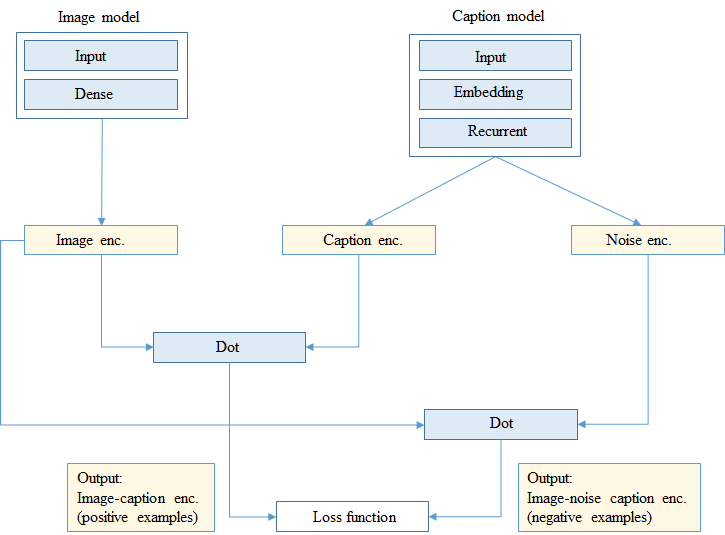
\includegraphics[scale=.6]{figures/arc2.png}
\caption{Image caption retrieval model}
\label{fig:img_cap_model}
\end{figure}

\justify
\textbf{\textit{Note:}}

\justify
To train the model, you will need to sample one caption per image (data originally contains five captions per image). You also need to create noise pairs of image and caption. 

\subsection*{Task 3.2: Caption retrieval}

Given an image (file path of the image) as a query, retrieve ten (10) possible captions of that image. Present the similarity score for the retrieved captions. Briefly discuss the result.

\subsection*{Task 3.3: Image retrieval}

Given a text query, retrieve ten (10) images correspond to that text. Present the similarity score of the retrieved images and its original caption. Discuss the result.

\justify
\textbf{\textit{Note:}}

\justify
Consider to use the following settings for image retrieval task. 

\begin{itemize}
    \item use real caption that is available in validation set as a query.
    \item use part of caption as query. For instance, instead of use the whole text sentence of the caption, you may consider to use key phrase or combination of words that is included in corresponding caption. 
\end{itemize}

\end{document}